% Vorbereitung: Vorbereitungsaufgaben bearbeiten
% Versuchsaufbau: Verwendete Apparatur, Beschreibung Funktionsweise/Nutzen mit Skizze/Foto
\section{Durchführung}
\label{sec:durchführung}

In der Abbildung ist der verwendete Aufbau für den Versuch zur Bestimmung der Reichweite von $\alpha$-Teilchen zu sehen.
\begin{figure}[H]
	\centering
    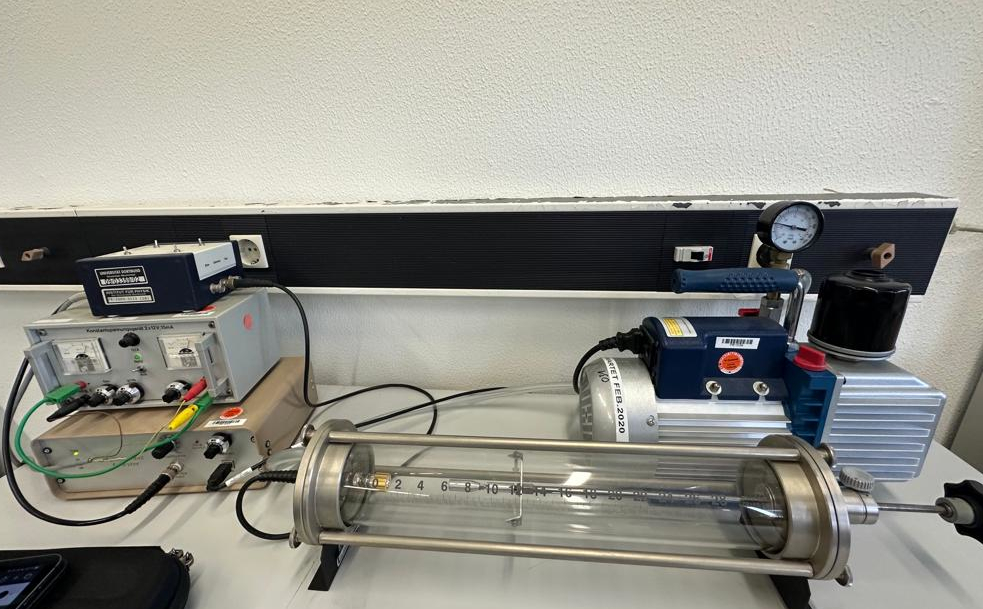
\includegraphics[width=0.75\linewidth]{content/grafik/aufbau.jpg}
    \caption{Der Versuchsaufbau zur Bestimmung der Reichweite von $\alpha$-Teilchen.}
    \label{fig:aufbau}
\end{figure}
In einem evakuierten Glaszylinder befindet sich das $\alpha$-Präparat un dein Detektor. Mittels einer Vakuumpumpe
wird der Glaszylinder evakuiert, sodass zum Start der ersten Messung ein Druck von $\SI{0}{mbar}$ herrscht.
Als Strahlungsquelle wird ein Am-Präparat verwendet. Dieses zerfällt mit einer Halbwertszeit von $ \symup{T}_{1/2} = 459 a$ in
\begin{equation*}
    \ce{^{241}_95Am -> ^{237}_93N + ^4_2He^{++}} .
\end{equation*}
Das Präparat befindet sich an einem verschiebbaren Regler, sodass es möglich ist einen Abstand $x$ zum Detektor
einzustellen. Als Detektor wird ein Hableiter-sperrschichtzähler verwendet.

Bevor der Versuch durchgeführt werden kann, muss der Aufbau und dessen Verkabelung überprüft werden.
Die Probe wird zunächst mit einem Abstand von $\SI{6}{\centi\meter} $ zum Detektor eingestellt. Der Glaszylinder
wird evakuiert mit Hilfe der Vakuumpumpe. Das Programm, welches zur Messung der $\alpha$-Teilchen verwendet wird, wird geöffnet.
Es wird die Schalterstellung $AUTO$ auf 2 Minutren eingestellt. Sobald die Messung gestartet wird, misst das Programm die 
Häufigkeit der Energien, die die Helium Kerne besitzen. Ausgegeben werden die Anzahl der detektierten $\alpha$-Teilchen, die 
Energien derer und die Häufigkeite derer. Nach den 2 Minuten wird der Druck im Glaszylinder um $\SI{50}{\mbar}$ erhöht. Dieser
Vorgang wird wiederholt bis keine Teilchen mehr detektiert werden oder bis der Druck $\SI{1}{\mbar}$ erreicht hat.
Für den zweiten Durchlauf der Messung wurde ein Abstand von $\SI{4}{\centi\meter}$ eingestellt. Dieser wurde solange
durchgeführt bis keine Teilchen mehr nachgewiesen werden konnten.

Nach den zwei Messdurchgängen wird ein konstanter Druck von $\SI{300}{\mbar}$ eingestellt und ein fester Abestand von $\SI{4}{\centi\meter}$ wird gewählt.
Es wird ein fester Zeitraum vom $\SI{10}{\second}$ eingestellt, indem gemessen wird. Dies wird 100 mal wiederholt.

